\documentclass{beamer}

\usepackage{graphicx}
\usepackage{graphics}
\usepackage{hyperref}
\usepackage[french]{babel}
\usepackage[utf8]{inputenc}
\usepackage[T1]{fontenc}
\usepackage{listings}

\graphicspath{{res/}}
\lstset{language=bash,basicstyle=\rm\small\ttfamily}

\newenvironment{wideitemize}{\itemize\addtolength{\itemsep}{10pt}}{\enditemize}

\mode<presentation>
	{
	\usetheme{epl}
	%\usetheme{Pittsburgh}
	\setbeamercovered{transparent = 28}
	}

\title{Contribuer aux synthèses}
\subtitle{GitHub EPL}
\author{Florian Thuin}
\institute{École Polytechnique de Louvain}

\begin{document}

\begin{frame}[plain]
	\titlepage
\end{frame}


\AtBeginSection[]
{
   \begin{frame}
       \frametitle{Sommaire}
       \tableofcontents[currentsection]
   \end{frame}
}

\section{Présentation de synthèses EPL}

\begin{frame}
	\frametitle{Qu'est-ce que synthèses EPL?}
		\begin{itemize}
 			\item \href{https://github.com/Gp2mv3/Syntheses}{Un répertoire sur GitHub} permettant aux étudiants de
 			    partager des résumés, des examens, des notes de cours,
 			    des résolutions d'exercices,\ldots
 			\item Contient des documents utiles pour tous les étudiants
 			    de l'École Polytechnique de Louvain
 			\item Un nombre limité de personnes s'assure de la gestion
 			    correcte du dossier et surveille les changements et
 			    améliorations pour maintenir la qualité sur le répertoire
 			    principal
 		\end{itemize}
\end{frame}

\section{Installer \texttt{git}}

\begin{frame}[fragile]
    \frametitle{Installation de \lstinline|git|}
    \begin{description}
        \item[Linux-Debian] En console : \lstinline|sudo apt-get install git|
        \item[Linux-Fedora] En console : \lstinline|sudo yum install git|
        \item[macOS] Tapez \lstinline|git| en console, cela lancera
            l'installation par Xcode (macOS 10.9 et supérieur).
        \item[Windows] Build officiel à l'adresse
            \url{http://git-scm.com/download/win}
    \end{description}
    \begin{itemize}
        \item Si vous ne maitrisez pas l'utilisation de \lstinline|git|, vous pouvez
            vous référer à
            \href{http://sites.uclouvain.be/SystInfo/notes/Outils/html/git.html}{ce
            tutoriel de Benoît Legat}
    \end{itemize}
\end{frame}

\section{Faire un fork du dossier de synthèses}

\begin{frame}
	\frametitle{Avoir les synthèses sur son propre compte}
		\begin{wideitemize}
			\item Se connecter à \lstinline|git|
			\pause
			\item Se rendre à l'adresse
                \url{https://github.com/Gp2mv3/Syntheses}
			\pause
			\item Cliquer sur Fork
                \begin{figure}[H]
                    \centering
                    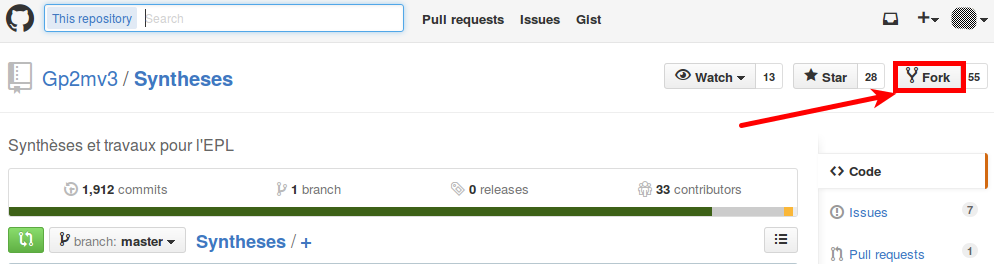
\includegraphics[width=\linewidth]{fork.png}
                \end{figure}
			\pause
			\item Vous disposez maintenant de votre copie du répertoire
		\end{wideitemize}
\end{frame}

\section{Cloner le répertoire contenant le fork}

\begin{frame}[fragile]
    \frametitle{Avoir le dossier des synthèses sur son ordinateur}
    \begin{wideitemize}
        \item Se connecter à \lstinline|git|
        \pause
        \item Écrire la commande suivante dans la console :
            \lstinline[mathescape]|git clone https://github.com/pseudonym/Syntheses.git| \textbf{en changeant \lstinline|pseudonym| par votre propre nom d'utilisateur}.
        \pause
        \item Vous disposez maintenant d'une copie synchronisée des
            synthèses.
    \end{wideitemize}
\end{frame}

\section{Installation et utilisation de \LaTeX}

\begin{frame}[fragile]
    \frametitle{Installation et utilisation de \LaTeX}
    \begin{itemize}
        \item Assurez-vous d'avoir une bonne connexion Internet
    \end{itemize}
    \begin{description}
        \item[Linux] \lstinline|sudo apt-get install texlive-full|
        \item[macOS] Télécharger \lstinline|MacTex.pkg|
            \url{http://www.tug.org/mactex/mactex-download.html}
        \item[Windows] Installer MiKTeX \url{http://miktex.org/download}
            et installer un éditeur de texte type TeXnicCenter
            \url{http://www.texniccenter.org/download/}
    \end{description}
    \begin{itemize}
        \item
            \href{https://github.com/blegat/LaTeXconf/blob/master/main.pdf}{Formation
            par Benoît Legat}
        \item
            \href{http://www.latex-howto.be/files/LaTeX-HowTo-full.pdf}{Livre
            de référence de qualité par Sébastien Combéfis}
    \end{itemize}
\end{frame}

\section{Contenu des sous-dossiers}

\subsection{Création et contenu des synthèses}

\begin{frame}
    \frametitle{Les synthèses - la classe Summary}
    \begin{exampleblock}{\textbf{À la racine}, exécutez \lstinline|add.sh| en
    console de cette manière :}
       \begin{tabular}{lllllll}
           \lstinline|bash| & \lstinline|add.sh| & quadri & titre & sigle & code & type d'ajout
           \\ \hline
           \lstinline|bash| & \lstinline|add.sh| & \lstinline|1| & \lstinline|math| & \lstinline|FSAB| & \lstinline|1101| & \lstinline|summary| \\
       \end{tabular}
    \end{exampleblock}
    \bigskip

    \begin{itemize}
        \item Document synthétique reprenant le cours de manière globale
        \item Ne suit pas forcément la structure du cours
        \item Suppose une compréhension préalable de la matière par le
            lecteur
        \item Structure claire et concise permettant une étude rapide
            mais pas nécessairement pédagogique
    \end{itemize}
\end{frame}

\subsection{Création et contenu des notes}

\begin{frame}
    \frametitle{Les notes - la classe Notes}
    \begin{exampleblock}{\textbf{À la racine}, exécutez \lstinline|add.sh| en
    console de cette manière :}
       \begin{tabular}{lllllll}
           \lstinline|bash| & \lstinline|add.sh| & quadri & titre & sigle & code & type d'ajout
           \\ \hline
           \lstinline|bash| & \lstinline|add.sh| & \lstinline|1| & \lstinline|math| & \lstinline|FSAB| & \lstinline|1101| & \lstinline|notes| \\
       \end{tabular}
    \end{exampleblock}
    \bigskip

    \begin{itemize}
        \item Suit la structure du cours
        \item Vient en complément des supports de cours officiels
            (syllabus et slides)
        \item Apporte des explications supplémentaires
        \item Pas forcément synthétique
        \item Pas forcément exhaustif
        \item La structure doit permettre au lecteur d'utiliser les
            notes pour une lecture annexe à celle des autres supports
    \end{itemize}
\end{frame}

\subsection{Création et contenu des examens et des tests}

\begin{frame}
    \frametitle{Les examens et test - Classe Exam et Test}
    \begin{exampleblock}{\textbf{À la racine}, exécutez \lstinline|add.sh| en
    console de cette manière :}
       \tiny \begin{tabular}{lllllllllll}
           \lstinline[basicstyle=\rm\tiny\ttfamily]|bash| & \lstinline[basicstyle=\rm\tiny\ttfamily]|add.sh| & quadri & titre & sigle & code & type & sol &
           year & month & minmaj \\
           \hline
	   \lstinline[basicstyle=\rm\tiny\ttfamily]|bash| &
	   \lstinline[basicstyle=\rm\tiny\ttfamily]|add.sh| &
	   \lstinline[basicstyle=\rm\tiny\ttfamily]|1| & \lstinline[basicstyle=\rm\tiny\ttfamily]|math|
	   & \lstinline[basicstyle=\rm\tiny\ttfamily]|FSAB| &
	   \lstinline[basicstyle=\rm\tiny\ttfamily]|1101| &
	   \lstinline[basicstyle=\rm\tiny\ttfamily]|test| &
	   \lstinline[basicstyle=\rm\tiny\ttfamily]|both| &
	   \lstinline[basicstyle=\rm\tiny\ttfamily]|2015| &
	   \lstinline[basicstyle=\rm\tiny\ttfamily]|Novembre| &
	   \lstinline[basicstyle=\rm\tiny\ttfamily]|All| \\
	   \lstinline[basicstyle=\rm\tiny\ttfamily]|bash| &
	   \lstinline[basicstyle=\rm\tiny\ttfamily]|add.sh| &
	   \lstinline[basicstyle=\rm\tiny\ttfamily]|4| & \lstinline[basicstyle=\rm\tiny\ttfamily]|fem|
	   & \lstinline[basicstyle=\rm\tiny\ttfamily]|MECA| &
	   \lstinline[basicstyle=\rm\tiny\ttfamily]|1120| &
	   \lstinline[basicstyle=\rm\tiny\ttfamily]|test| &
	   \lstinline[basicstyle=\rm\tiny\ttfamily]|only| &
	   \lstinline[basicstyle=\rm\tiny\ttfamily]|2013| &
	   \lstinline[basicstyle=\rm\tiny\ttfamily]|Avril| &
	   \lstinline[basicstyle=\rm\tiny\ttfamily]|Mineure| \\
	   \lstinline[basicstyle=\rm\tiny\ttfamily]|bash| &
	   \lstinline[basicstyle=\rm\tiny\ttfamily]|add.sh| &
	   \lstinline[basicstyle=\rm\tiny\ttfamily]|6| &
	   \lstinline[basicstyle=\rm\tiny\ttfamily]|oz| &
	   \lstinline[basicstyle=\rm\tiny\ttfamily]|INGI| &
	   \lstinline[basicstyle=\rm\tiny\ttfamily]|1131| &
	   \lstinline[basicstyle=\rm\tiny\ttfamily]|test| &
	   \lstinline[basicstyle=\rm\tiny\ttfamily]|none| &
	   \lstinline[basicstyle=\rm\tiny\ttfamily]|2015| &
	   \lstinline[basicstyle=\rm\tiny\ttfamily]|Mars| &
	   \lstinline[basicstyle=\rm\tiny\ttfamily]|Majeure| \\
       \end{tabular}
    \end{exampleblock}
    \begin{itemize}
        \item Destiné à contenir soit les questions d'examens soit les
            questions des tests
            \begin{itemize}
                 \item Ne contient que les questions (\lstinline|sol=none|)
                 \item Ne contient que les réponses (\lstinline|sol=only|)
                 \item Contient les questions et les réponses (\lstinline|sol=both|)
             \end{itemize}
    \end{itemize}
\end{frame}

\subsection{Création et contenu des choix multiples}

\begin{frame}
    \frametitle{Les choix multiples - Classe MCQ}
    \begin{exampleblock}{\textbf{À la racine}, exécutez \lstinline|add.sh| en
    console de cette manière :}
       \begin{tabular}{lllllll}
           \lstinline|bash| & \lstinline|add.sh| & quadri & titre & sigle & code & type d'ajout
           \\ \hline
           \lstinline|bash| & \lstinline|add.sh| & \lstinline|4| & \lstinline|eco| & \lstinline|FSAB| & \lstinline|1803| & \lstinline|mcq| \\\\
       \end{tabular}
    \end{exampleblock}
    \begin{itemize}
        \item Permet de créer des suites de propositions évaluables à
            VRAI ou FAUX avec la possibilité d'une justification
        \item Pouvant être avec ou sans réponse, avec ou sans
            justification.
    \end{itemize}
\end{frame}


\subsection{Création et contenu des exercices}

\begin{frame}
    \frametitle{Les exercices - Classe Exercises}
    \begin{exampleblock}{\textbf{À la racine}, exécutez \lstinline|add.sh| en
    console de cette manière :}
       \begin{tabular}{lllllllllll}
           \lstinline|bash| & \lstinline|add.sh| & quadri & titre & sigle & code & type & sol \\
           \hline
	   \lstinline|bash| & \lstinline|add.sh| & \lstinline|1| & \lstinline|math| & \lstinline|FSAB| & \lstinline|1101| & \lstinline|exercises| & \lstinline|both| \\
	   \lstinline|bash| & \lstinline|add.sh| & \lstinline|2| & \lstinline|math| & \lstinline|FSAB| & \lstinline|1102| & \lstinline|exercises| & \lstinline|only| \\
	   \lstinline|bash| & \lstinline|add.sh| & \lstinline|3| & \lstinline|math| & \lstinline|FSAB| & \lstinline|1103| & \lstinline|exercises| & \lstinline|none| \\
       \end{tabular}
   \end{exampleblock}
   \begin{itemize}
       \item Destiné à contenir les énoncés et les réponses des séances
           d'exercices
           \begin{itemize}
               \item Ne contient que les questions (\lstinline|sol=none|)
               \item Ne contient que les réponses (\lstinline|sol=only|)
               \item Contient les questions et les réponses (\lstinline|sol=both|)
       \end{itemize}
   \end{itemize}

\end{frame}

\section{Proposer une pull request}

\begin{frame}
    \frametitle{Proposer ses changements au repository principal}
    \begin{wideitemize}
        \item Se rendre sur sa copie personnelle des synthèses
        \pause
        \item Comparer une pull request
            \begin{figure}[H]
                \centering
                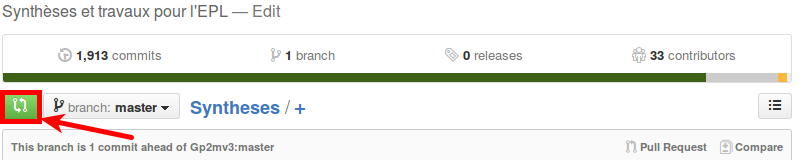
\includegraphics[width=\linewidth]{pull_request.png}
            \end{figure}
         \pause
         \item Proposer la pull request
            \begin{figure}[H]
                \centering
                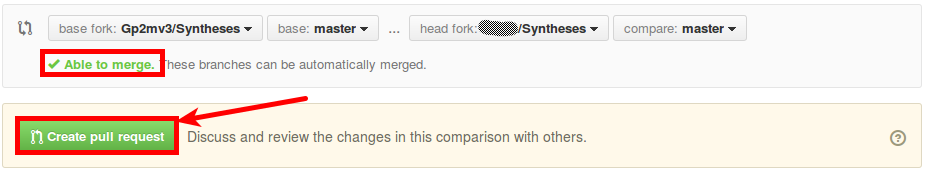
\includegraphics[width=\linewidth]{create_pull_request.png}
            \end{figure}
         \pause
         \item Donnez une explication sur le contenu de votre pull request
     \end{wideitemize}
\end{frame}

\section{Contribuer sans connaître \texttt{git}}

\begin{frame}
    \frametitle{Contribuer sans connaître GitHub - Les issues}
    \begin{itemize}
        \item Ma\^itriser un outil comme \lstinline|git| est indispensable dans le
            cadre de votre formation d'informatique pour participer à
            certains cours et contribuer à des projets avec les autres
            étudiants.
        \item Cependant, \lstinline|git| a prévu que vous puissiez signaler des
            problèmes que vous ne savez pas corriger vous-même, ça
            s'appelle \href{https://github.com/Gp2mv3/Syntheses/issues}{les issues}
    \end{itemize}
\end{frame}.

\end{document}
